\documentclass[IntroMain.tex]{subfiles} 
\begin{document}
	



\begin{frame}
	\frametitle{Binomial Probability Distribution}
	\Large
	A binomial experiment is one that possesses the following properties:
	
	1.   The experiment consists of n repeated trials;
	
	
	
	2.   Each trial results in an outcome that may be classified as a success or a failure (hence the name, binomial);
	
	
	
	3.   The probability of a success, denoted by p, remains constant from trial to trial and repeated trials are independent.
	
\end{frame}
%=======================================================================================================%
\begin{frame}
	\frametitle{Binomial Probability Distribution}
	\Large
	
	The number of successes X in n trials of a binomial experiment is called a binomial random variable.
	
	The probability distribution of the random variable X is called a binomial distribution, and is given by the formula:
	
	
	P(X) = Cnx pxqn−x
	
	where
\end{frame}
%=======================================================================================================%
\begin{frame}
	\frametitle{Binomial Probability Distribution}
	\Large	
	n = the number of trials
	
	x = 0, 1, 2, ... n
	
	p = the probability of success in a single trial
	
	q = the probability of failure in a single trial
	
	(i.e. q = 1 − p)
	
	Cnx is a combination value, found using the Choose operator.
	
\end{frame}
%=======================================================================================================%
\begin{frame}
	\frametitle{Binomial Probability Distribution}
	\Large
	
	P(X) gives the probability of successes in n binomial trials.
	
	If p is the probability of success and q is the probability of failure in a binomial trial, then the expected number of successes in n trials (i.e. the mean value of the binomial distribution) is
	
	\[E(X) = \mu  = np\]
	
\end{frame}
%=======================================================================================================%
\begin{frame}
	\frametitle{Binomial Probability Distribution}
	\Large
	The variance of the binomial distribution is
	
	V(X) = σ2 = npq
	
	Note: In a binomial distribution, only 2 parameters, namely n and p, are needed to determine the probability.
	
	
	

\end{frame}	
%==================================================================================== %
\begin{frame}
	
	The Binomial Dsitributuion is characheterized by the following parameters
	
	
	
	1) N - the number of trials
	
	2) P - The probability of a "success"
	

\end{frame}	
%==================================================================================== %
\begin{frame}
	The word "success" means that the outcome is the outcome of interest.
	
	If the outcome of interest is something like a flat tire, using the word "success" is coutner intuituive.
	
	
	A binomial experiment (also known as a Bernoulli trial) is a statistical experiment that has the following properties:
	
	The experiment consists of n repeated trials.
	

\end{frame}	
%==================================================================================== %
\begin{frame}	
	Each trial can result in just two possible outcomes. We call one of these outcomes a success and the other, a failure.
	
	The probability of success, denoted by P, is the same on every trial.
	
	The trials are independent; that is, the outcome on one trial does not affect the outcome on other trials.
	
	


\end{frame}	
%==================================================================================== %
\begin{frame}	
	The Binomial Dsitributuion is characheterized by the following parameters
	
	
	
	1) N - the number of trials
	
	2) P - The probability of a "success"
	
	
	
	The word "success" means that the outcome is the outcome of interest.
	
	If the outcome of interest is something like a flat tire, using the word "success" is coutner intuituive.

\end{frame}	
%==================================================================================== %
\begin{frame}	
	A binomial experiment (also known as a Bernoulli trial) is a statistical experiment that has the following properties:
	
	The experiment consists of n repeated trials.
	
	
	Each trial can result in just two possible outcomes. We call one of these outcomes a success and the other, a failure.
	
	The probability of success, denoted by P, is the same on every trial.
	
	The trials are independent; that is, the outcome on one trial does not affect the outcome on other trials.
	
\end{frame}	
	
%==================================================================================== %	
\frame{
	\frametitle{The Binomial Probability Distribution}
	\begin{itemize}
		\item The number of independent trials is denoted $n$.
		\item The probability of a `success' is $p$
		\item The expected number of `successes' from $n$ trials is $E(X) = np$
	\end{itemize}
}	
%--------------------------------------------------------------------------------------%
\frame{
\frametitle{Binomial Experiment}
A binomial experiment (also known as a Bernoulli trial) is a statistical experiment that has the following properties:
\begin{itemize}
\item The experiment consists of $n$ repeated trials.
\item Each trial can result in just two possible outcomes. We call one of these outcomes a \textbf{\emph{success}} and the other, a \textbf{\emph{failure}}.
\item The probability of success, denoted by $p$, is the same on every trial.
\item The trials are independent; that is, the outcome on one trial does not affect the outcome on other trials.
\end{itemize}
}
%--------------------------------------------------------------------------------------%
\frame{
\frametitle{Binomial Experiment}
Consider the following statistical experiment. You flip a coin five times and count the number of times the coin lands on heads. This is a binomial experiment because:
\begin{itemize}
\item The experiment consists of repeated trials. We flip a coin five times.
\item Each trial can result in just two possible outcomes : heads or tails.
\item The probability of success is constant : 0.5 on every trial.
\item The trials are independent; that is, getting heads on one trial does not affect whether we get heads on other trials.
\end{itemize}
}
%--------------------------------------------------------------------------------------%
\frame{
\frametitle{Binomial Probability}
\begin{itemize}
\item A binomial experiment with n trials and
probability $p$ of success will be denoted by
\[B(n, p)\]
\item Frequently, we are interested in the \textbf{\emph{number of successes}} in a binomial experiment, not in the order in which they occur.
\item Furthermore, we are interested in the probability of that number of successes.
\end{itemize}

}
%--------------------------------------------------------------------------------------%
\frame{
\frametitle{Binomial Probability}
The probability of exactly k successes in a binomial experiment B(n, p) is given by
\[ P(X=k) = P(k \mbox{ successes }) = \;^nC_k  \times p^{k} \times (1-p)^{n-k}\]

\begin{itemize}
\item X: Discrete random variable for the number of successes (variable name)
\item $k$ : Number of successes (numeric value)
\begin{itemize}
\item  $P(X=k)$ ``probability that the number of success is $k$".
\end{itemize}
\item $n$ : number of independent trials
\item $p$ : probability of a success in any of the $n$ trial.
\item $1-p$ : probability of a failure in any of the $n$ trial.
\end{itemize}

}


%--------------------------------------------------------------------------------------%
\frame{
\frametitle{Binomial Example }

Suppose a die is tossed 5 times. What is the probability of getting exactly 2 fours?

\textbf{Solution:}

This is a binomial experiment in which \begin{itemize}\item a success is defined as an outcome of `4'. \item the number of trials is equal to $n=5$, \item the number of successes is equal to $k=2$,\item the number of failures is equal to 3, \item  the probability of success on a single trial is 1/6, \item  the probability of failure on a single trial is 5/6.\end{itemize}
}
%--------------------------------------------------------------------------------------%
\begin{frame}[fragile]
\frametitle{Binomial Example }

Therefore, the probability of getting exactly 2 fours is:

\[P(X=2) = ^5C_2 \times (1/6)^2 \times (5/6)^3 = 0.161\]

Remark: $^5C_2 = 10$\\
\bigskip


\end{frame}

%--------------------------------------------------------%

\frame{
\frametitle{Binomial Example}

\begin{center}
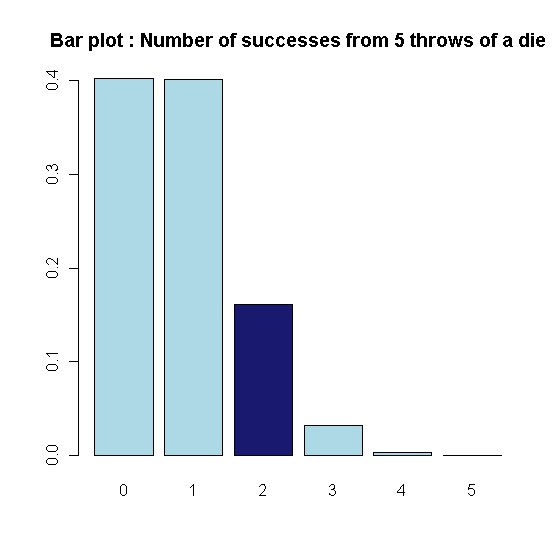
\includegraphics[scale=0.40]{images/3Bbarplot4}
\end{center}
}
%--------------------------------------------------------------------------------------%
\frame{
\frametitle{Binomial Probability}

\textbf{Remark} : The sum of the probabilities of each of the possible outcomes (i.e. no fours, one four etc) is equal to one.
\[P(X=0) + P(X = 1) + \ldots + P(X=5) = 1 \]

}
%--------------------------------------------------------%

\frame{
\frametitle{Binomial Example: At least two successes}
\begin{figure}
\centering
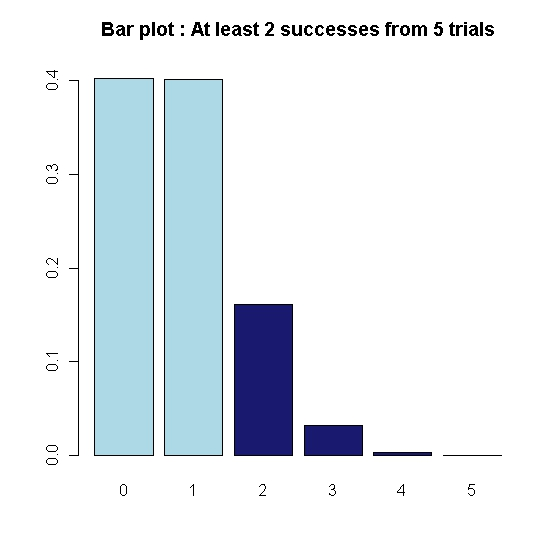
\includegraphics[width=0.7\linewidth]{images/3Bbarplot5}
\caption{}
\label{fig:3Bbarplot5}
\end{figure}

}

%--------------------------------------------------------%

\frame{
\frametitle{Binomial Example: At least two successes}
\begin{itemize}
\item Suppose we were asked to find the probability of \textbf{\emph{at least}} 2 fours.
\item Can you suggest the most efficient way of computing this?
\item Suggestion: Compute $P(X=0)$ and $P(X = 1)$.
\item Together these probabilities are the complement probability of what we require.
\item $P(X \geq 2) = 1 - ( P(X=0) + P(X = 1))$.
\item (We will continue with this in future classes).
\end{itemize}
}
%--------------------------------------------------------------------------------------%
\frame{
\frametitle{Cumulative Distribution Function}


The cumulative distribution function (c.d.f.) of a discrete random variable $X$ is the function $F(t)$ which tells you the probability that X is less than or equal to t. \\ So if X has p.d.f. P(X = x), we have:

\[ F(t) = P(X \leq t) = \sum_{(i=0)}^{(i=t)} P(X = x) \]

In other words, for each value that X can be which is less than or equal to $t$, work out the probability that X is that value and add up all such results.

}




%--------------------------------------------------------%

\begin{frame}[fragile]
\frametitle{Binomial Example: Sample Problem}

Suppose there are twelve multiple choice questions in an English class quiz. Each question has five possible answers, and only one of them is correct. Find the probability of having four or less correct answers if a student attempts to answer every question at random.
\end{frame}

%--------------------------------------------------------%

\begin{frame}[fragile]
	\frametitle{Binomial Example: Sample Problem}

\textbf{Solution:}
Since only one out of five possible answers is correct, the probability of answering a question correctly by random is $1/5=0.2$. We can find the probability of having exactly 4 correct answers by random attempts as follows.(Blackboard. Correct Answer is 13.29\%)
%\begin{verbatim}
%> dbinom(4, size=12, prob=0.2)
%[1] 0.1329
%\end{verbatim}
\end{frame}
%--------------------------------------------------------%


%--------------------------------------------------------------------------------------%
\frame{
	\frametitle{ Binomial Example 1 }
	(Revision from Last Class)\\
	Suppose a die is tossed 5 times. What is the probability of getting exactly 2 fours?
	
	\textbf{Solution:} This is a binomial experiment in which the number of trials is equal to 5, the number of successes is equal to 2, and the probability of success on a single trial is 1/6 or about 0.167. 
	\\
	\bigskip
	Therefore, the binomial probability is:
	
	\[P(X=2) = ^5C_2 \times (1/6)^2 \times (5/6)^3 = 0.161\]
}

%--------------------------------------------------------------------------------------%
\frame{
	\frametitle{ Binomial Example 2 }
	Suppose there is a container that contains 6 items.  The probability that any one of these items is defective is 0.3. Suppose all six items are inspected. 
	\begin{itemize}
		\item What is the probability of 3 defective components?
		\item What is the probability of 4 defective components?
	\end{itemize}
	
	\[ P(3\text{ defects}) = f(3) = P(X = 3) = {6\choose 3}0.3^3 (1-0.3)^{6-3} = 0.1852 \]
	\[ P(4\text{ defects}) = f(4) = P(X = 4) = {6\choose 4}0.3^4 (1-0.3)^{6-4} = 0.0595 \]
}

%------------------------------------------------------------------%
\frame{
	\frametitle{Binomial Expected Value and Variance}
	
	
	If the random variable X has a binomial distribution with parameters n
	and p, we write
	\[ X \sim B(n,p) \]
	
	Expectation and Variance
	If $X \sim B(n,p)$, then:
	
	\begin{itemize}
		\item Expected Value of X : E(X) = np
		\item Variance of X : Var(X) = np(1-p)
	\end{itemize}
}
%---------------------------------------------------------------------%
\begin{frame}
	\frametitle{Binomial Distribution: Example 1}
	\begin{itemize} \item Diagrams of the probability mass functions of the two binomial
		distributions $B(10, 0.5)$ and $B(10, 0.25)$ are shown in the bar-plots (next slide). \item Which
		is which? Give a reason for your answer.
	\end{itemize}
\end{frame}
%---------------------------------------------------------------------%
\begin{frame}
	\frametitle{Binomial Distribution}
	\begin{figure}
		% Requires \usepackage{graphicx}
		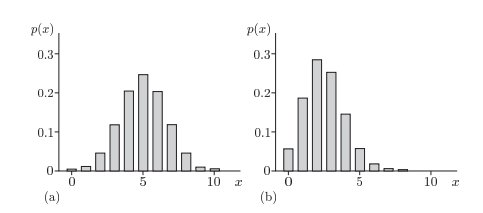
\includegraphics[scale=0.60]{images/4ABarCharts.jpg}\\
		\caption{Bar Charts}
	\end{figure}
\end{frame}
%---------------------------------------------------------------------%
\begin{frame}
	\frametitle{Binomial Distribution: Example 1}
	\begin{itemize}
		\item Clearly. Figure A is $B(10, 0.5)$ and Figure B is $B(10, 0.25)$.
		\item The mean of B(10, 0.5) is 5, and the mean of B(10, 0.25) is 2.5. These values correspond to the apex of both distributions on the previous slide.
		\item Also the variance of a binomial distribution corresponding to $B(10, 0.25)$ is $1.875$, while for $B(10, 0.25)$ it is $2.500$.
		\item A visual inspection of the two bar-charts would indicate that Figure A has the higher variance.
	\end{itemize}
\end{frame}
%---------------------------------------------------------------------%
\begin{frame}
	\frametitle{Binomial Distribution: Example 2}
	\textbf{Example}
	\begin{itemize}
		\item Components are placed into containers containing 100 items.
		\item After an inspection of a large number of containers the average number of defective items was found to be 10 with a standard deviation of three.
		\item Is the binomial distribution a good useful distribution, given the observed data?
	\end{itemize}
\end{frame}
%---------------------------------------------------------------------%
\begin{frame}
	\frametitle{Binomial Distribution: Example 2}
	
	\begin{itemize}
		\item Let the number of containers be the number of independent trials is $n=100$.
		\item A success may be defined as a defective component.
		\item The probability of a success is approximate $p=0.10$. (The probability of ``failure" is $1-p=0.9$).
		\item The expected number of defective components is $np=10$, which concurs with our observed data.
		\item The variance is computed as \[np(1-p) = 100 \times 0.1 \times 0.9 = 9\]
		\item The observed standard deviation is 3 units, i.e. a variance of 9 square units.
		\item Yes the binomial distribution is useful in this case.
	\end{itemize}
\end{frame}
%============================================================ %
\begin{frame}
	The Binomial distribution is a discrete distribution used.
	
	
	The outcome of interest is known as a `success'. If we are
	interested in how many times we get a six when a dice is rolled.
	
	The probability of success is denoted $p$.
	
	binomial coefficients
	\[
	\left( {\begin{array}{*{20}c} n \\ k \\ \end{array}} \right) =
	\frac{{n!}}{{k!\left( {n - k} \right)!}} \]
\end{frame}
%============================================================ %
\begin{frame}
	binomial probability
	\[y = \frac{{n!}}{{k!\left( {n - k} \right)!}}p^k q^{n - k} = \left( {\begin{array}{*{20}c} n \\ k \\ \end{array}} \right)p^k q^{n -
		k}\]
	
	mean and variance of Binomial distribution
	
	$M_{bin} = np$  and $\sigma ^2 _{bin} = np(1-p)$
	
	For example, if the sample size is 12 and the probability of
	success is 0.25, the mean is $12 \times 0.25 = 3$ and the variance
	is $\sigma ^2 _{bin} = 12 \times 0.25 \times 0.75 = 2.25$.
\end{frame}



\end{document}







